
\begin{figure}
 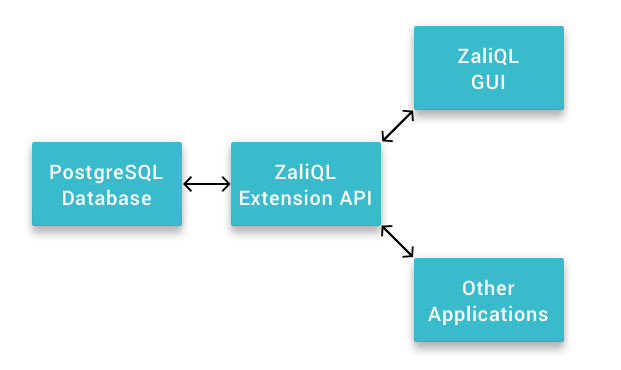
\includegraphics[scale=0.25]{Figures/System-Overview.png}
 \caption{\GSQLB\'s Architecture}
  \label{fig:arch}
  \vspace{-3mm}
\end{figure}

\begin{figure}
\hspace*{.3cm}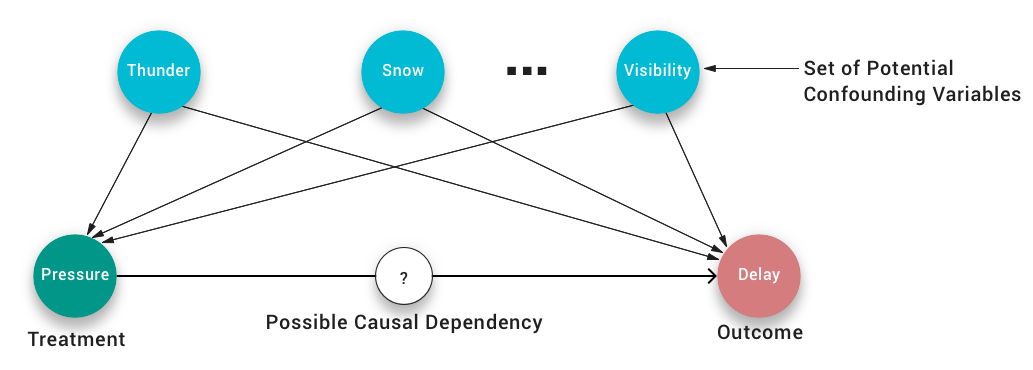
\includegraphics[scale=0.2]{figures/Scenario-Graph.png}
\caption{Confounding Influence \dans{move this figure later.}}

\label{fig:cv}
\vspace{-0.3cm}
\end{figure}

\section{System's Architecture}

The overall architecture of \GSQL\ is shown in Figure \ref{fig:arch}.
\dans{start by saying that data is stored in a Postgres system}
The API consists of a set of stored procedures which supports a wide range of methods for performing causal inference.  They are written in PL/pgSQL and are optimized for PostgreSQL. \footnote{\url{http://postgresql.org/}}
The API will be packed  as an extension of  PostgreSQL and will be released in 
PostgreSQL Extension Network.\footnote{\url{http://pgxn.org/}}
The functionality of the API is modeled after the MatchIt and CEM R libraries \cite{ho2005,iacus2009cem}. The web GUI (see Figure \ref{fig:eteresult}) is designed to wrap around \GSQL. It can be configured with the user's databases URL after they have installed the \GSQL\ Postgres extension. The  GUI be hosted remotely on a server or locally on your machine. \ignore{
The interface consists of three tabs : Setup, Matching Summary, and Analysis.
}

\dans{We should add more details here: describe the main functions
  that the API supports; mention that they generate and optimize SQL
  queries.}
